\documentclass{article}
\usepackage[margin=1.25in]{geometry}
\usepackage{amsmath, amssymb, setspace, enumerate, enumitem}
\usepackage{setspace}
\usepackage{graphicx}
\onehalfspacing

\begin{document}
    \begin{enumerate}
        \item \begin{enumerate}[label=(\alph*)]
            \item For the input point [2,1] and y = -1, with weights 0.15 applied. For identity: The first layer returns with results [ [0.2778125  0.2778125] [0.13890625 0.13890625] ] and layer two returns with results [[0.47529864] [0.47529864]]. For tanh: first layer w1: [[0.27569254 0.27569254][0.13784627 0.13784627]], second layer [[0.47167168][0.47167168]]. The $E_{in}(w)$ obtained was $0.3172898231266975$
            \item After peturbing the weights, I achieved the following: identity w1: [[0.27796641 0.27796641]
            [0.1389832  0.1389832 ]]
           w2: [[0.47564328]
            [0.47564328]] and tanh: w1: [[0.2758401  0.2758401 ]
            [0.13792005 0.13792005]]
           w2: [[0.47200485]
            [0.47200485]]. $E_{in}(w)$ was 0.31737905364130986\\[0.25in]
            As stated by the hint, after peturbing the weights, the results were relatively similar, only different in the final few digits, therefore we can conclude that our algorithm is correct.
        \end{enumerate}
        \item FINISH
        \item \begin{enumerate}[label=(\alph*)]
            \item We're given two two-dimensional inputs, $x_1 = (1,0)$ and $x_2 = (-1,0)$. The optimal separating hyperplane is simply a line. For SVM, we want to find the separator that maximizes the margin. Both of these lines depict a horizontal line with slope 0, the perpendicular bisector is the negative reciprocal of the line, which is a vertical line. A vertical line in $x = 0$ is our solution.
            \item \begin{enumerate}[label=(\roman*)]
                \item They are the same point $z_1 = (1,0)$ and $z_2 = (-1,0)$
                \item The same, $z = 0$ and it's a vertical line.
            \end{enumerate}
            \item 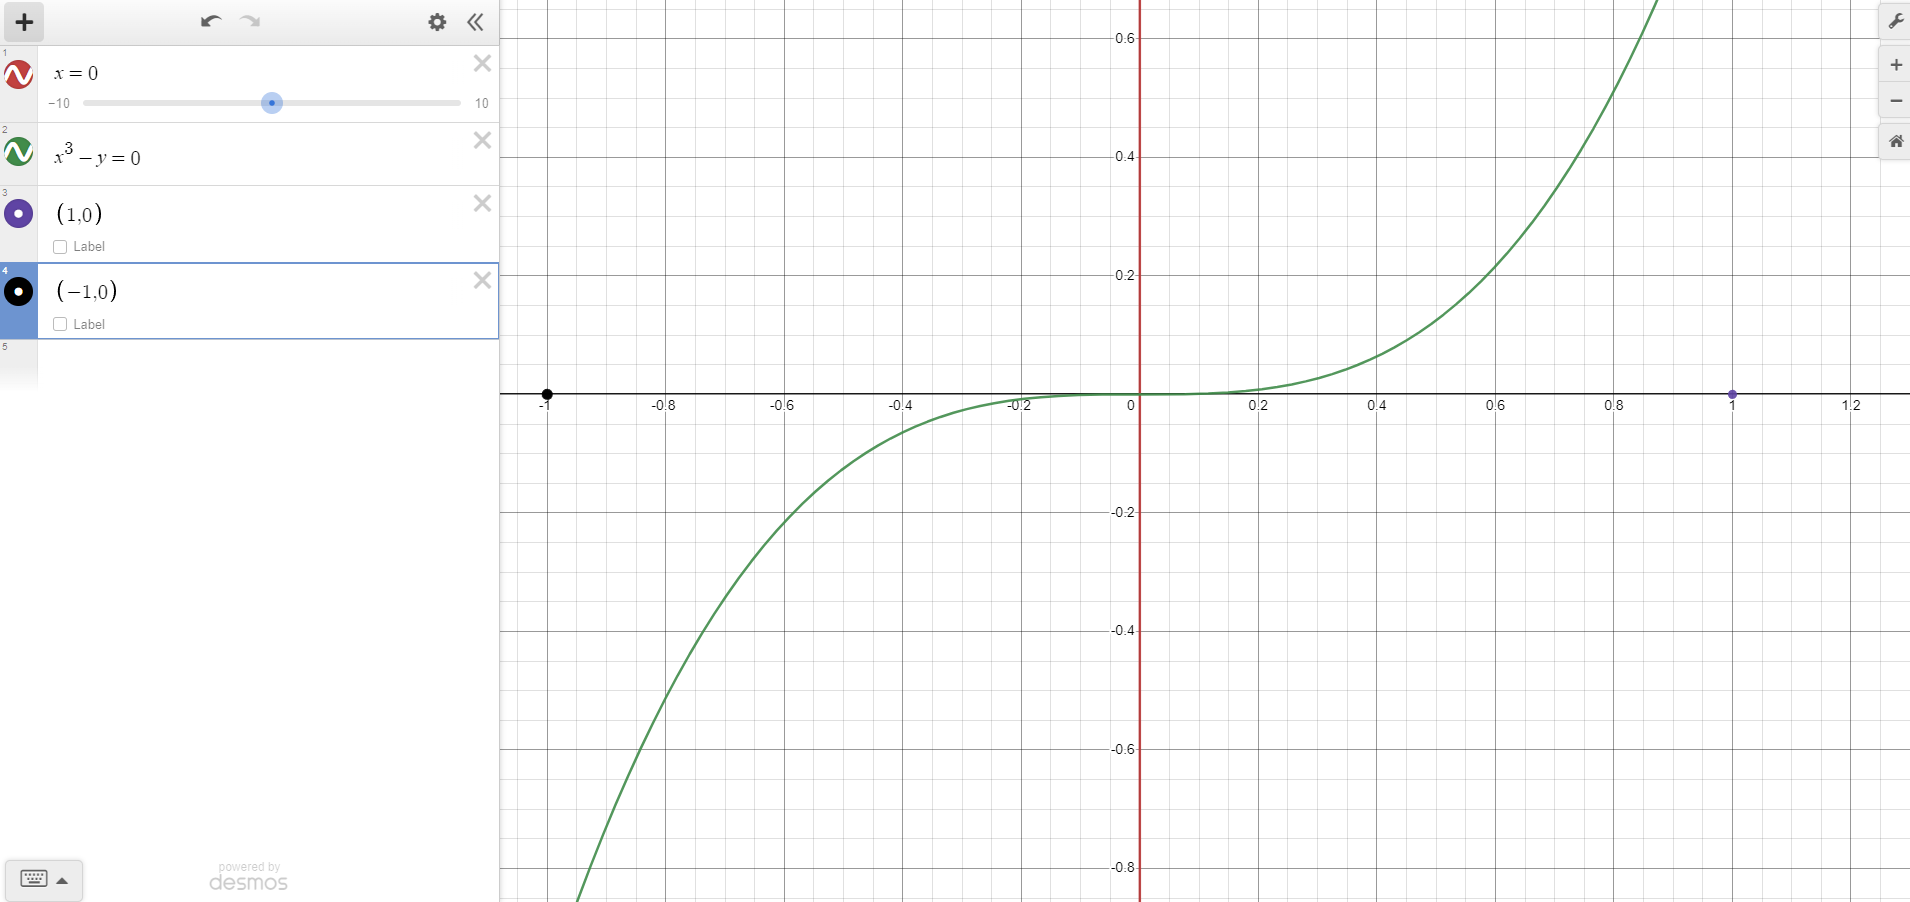
\includegraphics[scale=0.25]{images/3c.png}
            \item For $z(x) = \begin{bmatrix}
                    x^3_1 - x_2\\
                    x_1x_2
                \end{bmatrix}$, and $z(y) = \begin{bmatrix}
                    y^3_1 - y_2\\
                    y_1y_2
                \end{bmatrix}$, we can derive the following:
                \begin{align*}
                    K(x,y) &= z(x) \cdot z(y)\\
                    &= (x^3_1 - x_2)(y^3_1 - y_2) + (x_1x_2)(y_1y_2)\\
                    &= x^3_1y^3_1 - x^3_1y_2 - x_2y^3_1 + x_2y_2 + x_1x_2y_1y_2\\
                \end{align*}
            \item $h(x) = \text{sign}(x^3_1 - x_2 + x_1x_2)$
        \end{enumerate}
    \item FINISH
    \end{enumerate}
\end{document}